% !TEX TS-program = pdflatex
% !TEX encoding = UTF-8 Unicode

% This is a simple template for a LaTeX document using the "article" class.
% See "book", "report", "letter" for other types of document.

\documentclass[11pt]{article} % use larger type; default would be 10pt

\usepackage[utf8]{inputenc} % set input encoding (not needed with XeLaTeX)

%%% Examples of Article customizations
% These packages are optional, depending whether you want the features they provide.
% See the LaTeX Companion or other references for full information.

%%% PAGE DIMENSIONS
\usepackage{geometry} % to change the page dimensions
\geometry{a4paper} % or letterpaper (US) or a5paper or....
\geometry{margin=1in} % for example, change the margins to 2 inches all round
% \geometry{landscape} % set up the page for landscape
%   read geometry.pdf for detailed page layout information

\usepackage{graphicx} % support the \includegraphics command and options

% \usepackage[parfill]{parskip} % Activate to begin paragraphs with an empty line rather than an indent
\usepackage{amssymb}
\usepackage{amsmath}
%%% PACKAGES
\usepackage{booktabs} % for much better looking tables
\usepackage{array} % for better arrays (eg matrices) in maths
\usepackage{paralist} % very flexible & customisable lists (eg. enumerate/itemize, etc.)
\usepackage{verbatim} % adds environment for commenting out blocks of text & for better verbatim
\usepackage{subfig} % make it possible to include more than one captioned figure/table in a single float
% These packages are all incorporated in the memoir class to one degree or another...

%%% HEADERS & FOOTERS
\usepackage{fancyhdr} % This should be set AFTER setting up the page geometry
\pagestyle{fancy} % options: empty , plain , fancy
\renewcommand{\headrulewidth}{0pt} % customise the layout...
\lhead{}\chead{}\rhead{}
\lfoot{}\cfoot{\thepage}\rfoot{}

%%% SECTION TITLE APPEARANCE
\usepackage{sectsty}
\allsectionsfont{\sffamily\mdseries\upshape} % (See the fntguide.pdf for font help)
% (This matches ConTeXt defaults)

%%% ToC (table of contents) APPEARANCE
\usepackage[nottoc,notlof,notlot]{tocbibind} % Put the bibliography in the ToC
\usepackage[titles,subfigure]{tocloft} % Alter the style of the Table of Contents
\usepackage{bbm}
\usepackage{endnotes}

\renewcommand{\cftsecfont}{\rmfamily\mdseries\upshape}
\renewcommand{\cftsecpagefont}{\rmfamily\mdseries\upshape} % No bold!
\DeclareMathOperator*{\argmax}{arg\,max}
\DeclareMathOperator*{\argmin}{arg\,min}

\usepackage{graphicx}
\graphicspath{ {./pings/} }

\newcount\colveccount
\newcommand*\colvec[1]{
        \global\colveccount#1
        \begin{pmatrix}
        \colvecnext
}
\def\colvecnext#1{
        #1
        \global\advance\colveccount-1
        \ifnum\colveccount>0
                \\
                \expandafter\colvecnext
        \else
                \end{pmatrix}
        \fi
}

\newcommand{\norm}[1]{\left\lVert#1\right\rVert}

\title{Econometrics HW3}
\author{Michael B. Nattinger\footnote{I worked on this assignment with my study group: Alex von Hafften, Andrew Smith, and Ryan Mather. I have also discussed problem(s) with Emily Case, Sarah Bass, Katherine Kwok, and Danny Edgel.}}

\begin{document}
\maketitle

\section{Question 20.1}
For $X=3, Y = -1 +2X + 5X-5-3X+6+e$. Then, the marginal effect of $X$ on $Y$ for $X=3$ is $2+5-3 = 4$.
\section{Question 20.3}
For $m_k(x)$ to be concave then the slopes in all regions must be weakly decreasing:
\begin{align*}
\beta_1\geq \beta_1+\beta_2\geq \beta_1+\beta_2+\beta_3&\geq\beta_1+\beta_2+\beta_3+\beta_4\\
\Rightarrow \beta_2\leq0,\beta_3\leq0,\beta_4&\leq0.
\end{align*}
\section{Question 20.11} %stata
\subsection{Part A}
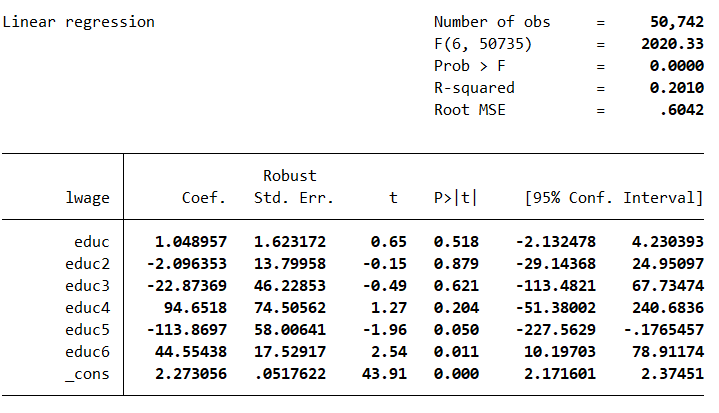
\includegraphics{p1}
\subsection{Part B}
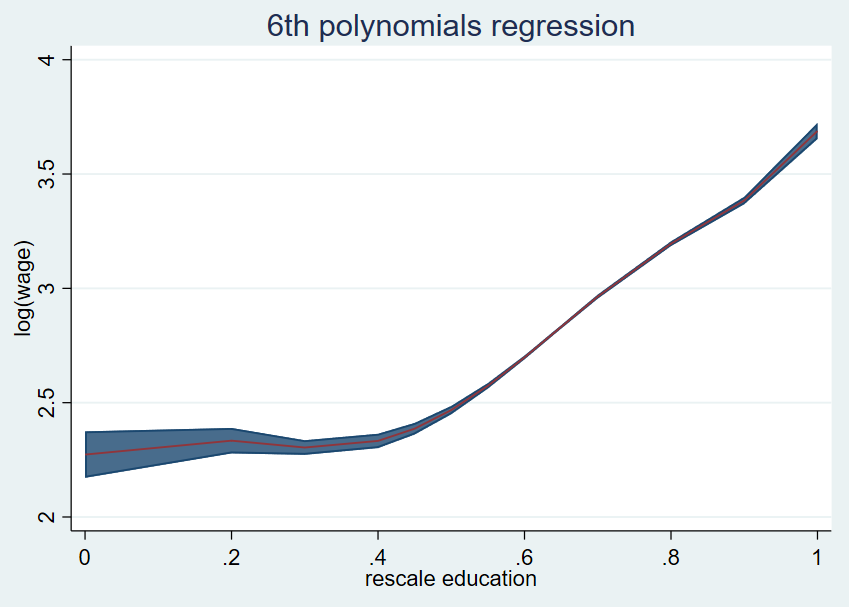
\includegraphics[scale=0.7]{p2}\\
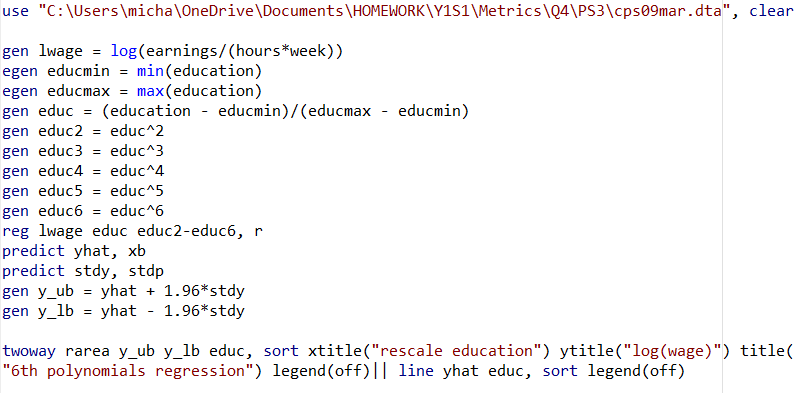
\includegraphics{p3}
\section{Question 20.15} %stata
\subsection{Part A}
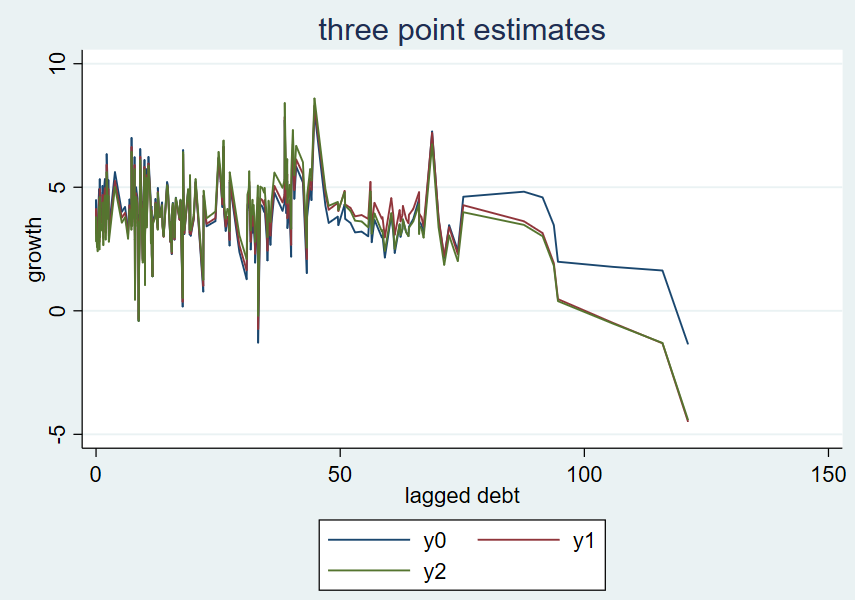
\includegraphics[scale=0.7]{p4}
\subsection{Part B}
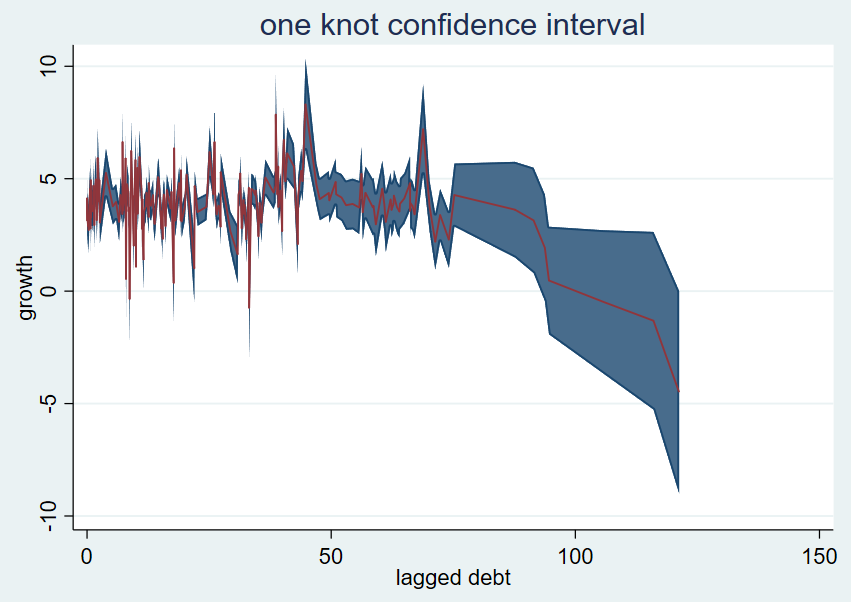
\includegraphics[scale=0.7]{p5}
\subsection{Part C}
The no-spline regression has an AIC of 1249.774, one-spline has an AIC of 1248.711, and two-spline has an AIC of 1248.688. The two-spline specification has the smallest AIC, so it has the preferred specification. One-spline is also preferred to no splines, and is very close to two-splines.
\subsection{Part D}
From the first figure we can see that there is a substantial drop off in growth for the observations with lagged debt above 90. This is consistent in all three models, and the effect is stronger in the two models with splines in the debt level. First, note that the two models with the more substantial drop-off have better AIC values than the model with the less substantial drop-off. Note also that this drop-off occurs at 90 for all models despite not having a spline at 90 for any of the model. The effect is just as pronounced in the model with the spline at 60 as it is with the splines at 40 and 80, despite the spline at 80 being substantially closer to 90 than the spline at 60. It should be noted, however, that the model is less precisely estimated near the drop-off point, which is evident in the second figure. In my opinion the drop off at 90 is quite substantial despite the reduced precision over this region.\\
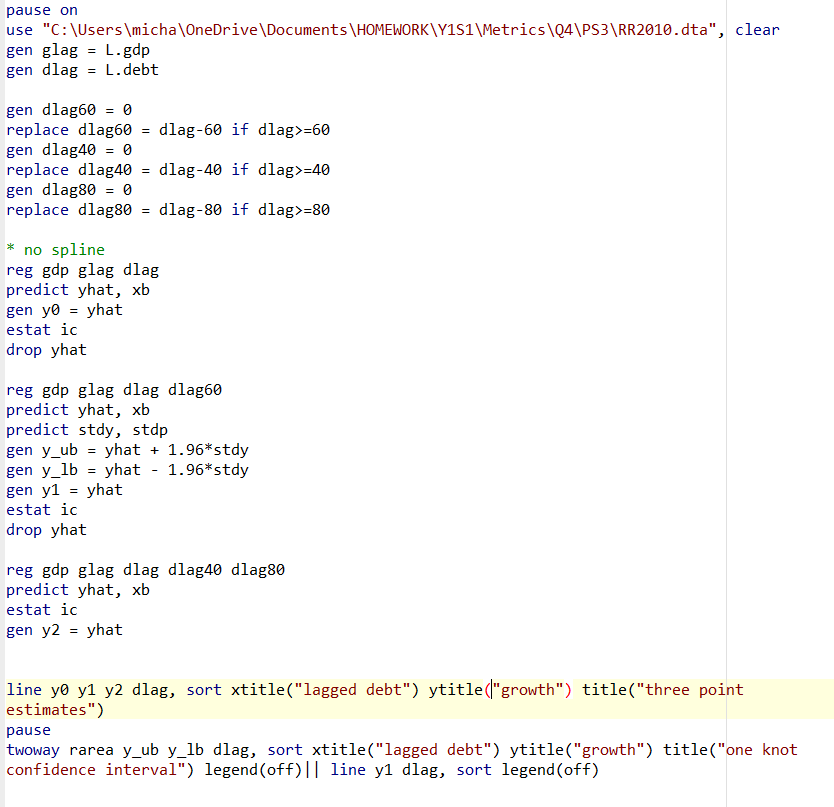
\includegraphics[scale=0.7]{p6}
\section{Question 21.1}
The difference is simply a sign difference. For $D'=1\{X\geq c \}$ we saw that $\bar{\theta}' = m(c+) - m(c-),$ but for $D = 1\{ X\geq c \}$ we now have $\bar{\theta} = m(c-) - m(c+)$.
\section{Question 21.2}
The identified treatment affects are at the end points $c_1,c_2$. We can identify $\bar{\theta}(c_1) = m(c_1+)-m(c_1-), \bar{\theta}(c_2) = m(c_2-) - m(c_2+)$.
\section{Question 21.3}
\begin{align*}
Y &= Y_01\{X<c\} + Y_11\{X\geq c\}\\
E[Y|X=x] &= E[Y_01\{X<c\}|X=x] + E[Y_11\{X\geq c\}|X=x]\\
m(x) &= m_0(x)1\{x<c\} + m_1(x)1\{x\geq c\}
\end{align*}
\section{Question 21.4}
With a rectangular kernel of appropriate bandwidth $2h$, $K\left(\frac{x - c}{2h}\right) = 1\{ |x - c| \leq h\}$. Then the local linear estimator objective function is the following:
\begin{align*}
J &= \sum_{i=1}^n (y_i - \beta_0 - \beta_1x_i - \beta_2(x_i-c)D_i - \theta D_i)^2K\left(\frac{x_i - c}{2h}\right)\\
&=  \sum_{i=1}^n (y_i - \beta_0 - \beta_1x_i - \beta_2(x_i-c)D_i - \theta D_i)^2 1\{ |x - c| \leq h\} \\
&=  \sum_{|x - c| \leq h} (y_i - \beta_0 - \beta_1x_i - \beta_2(x_i-c)D_i - \theta D_i)^2 
\end{align*}
This is the ols estimation on the appropriate subsample.
\section{Question 21.6} %stata
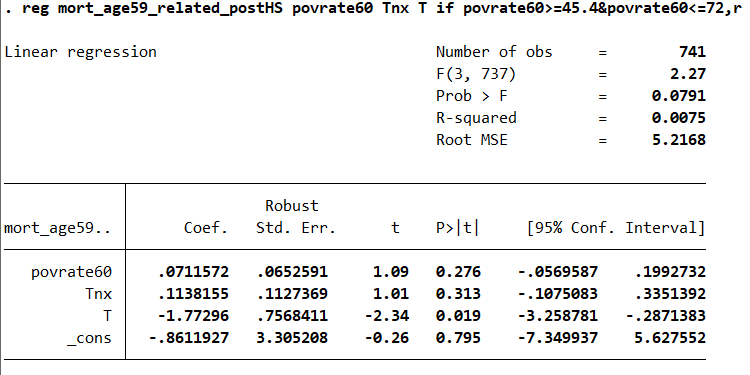
\includegraphics{p7}\\
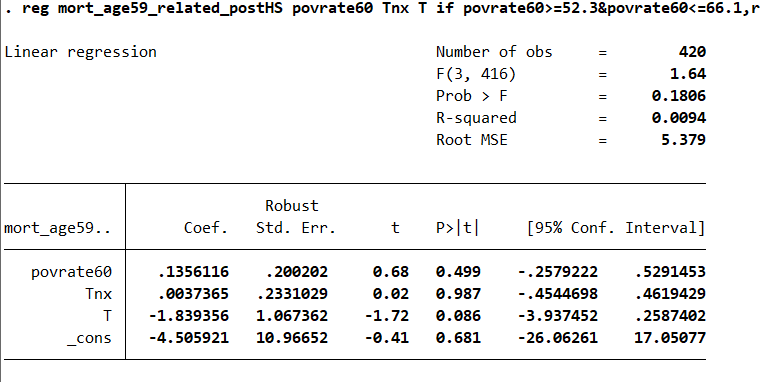
\includegraphics{p8}\\
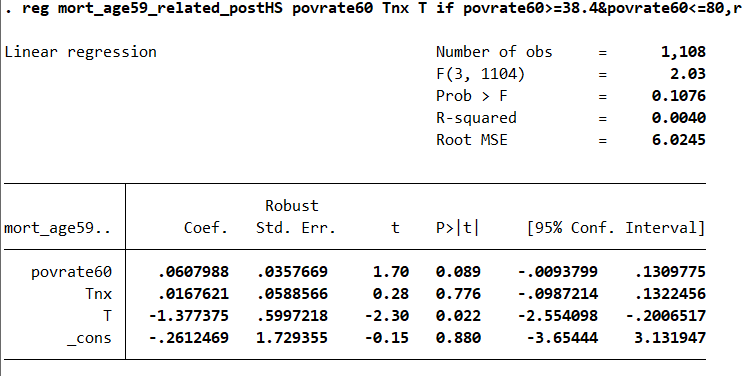
\includegraphics{p9}\\
The above regression outputes show the regression results from windows of $h = 8,4,12$, respectively. Note that $h=n$ corresponds to a bandwidth of $n\sqrt{3}$. The resulting coefficients $\bar{\theta}$, the coefficient on the variable $T$, are all of similar magnitude, and most are statistically significant, so the results are fairly robust to bandwidth.
\section{Question 21.8} %stata
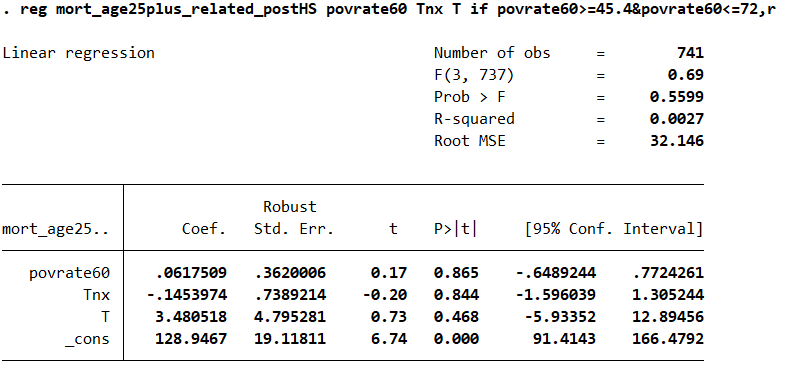
\includegraphics{p10}\\
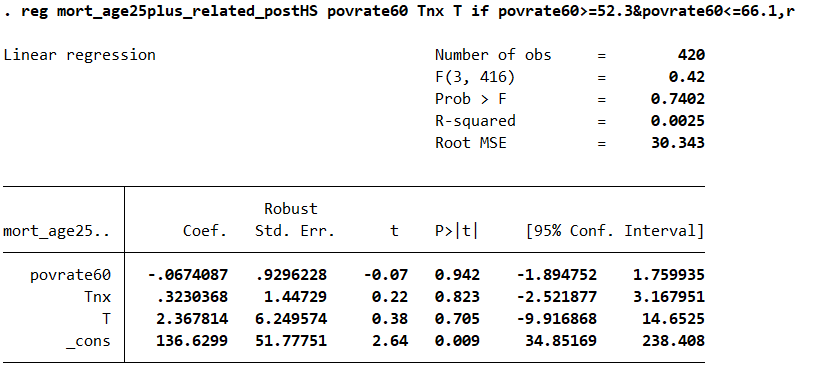
\includegraphics{p11}\\
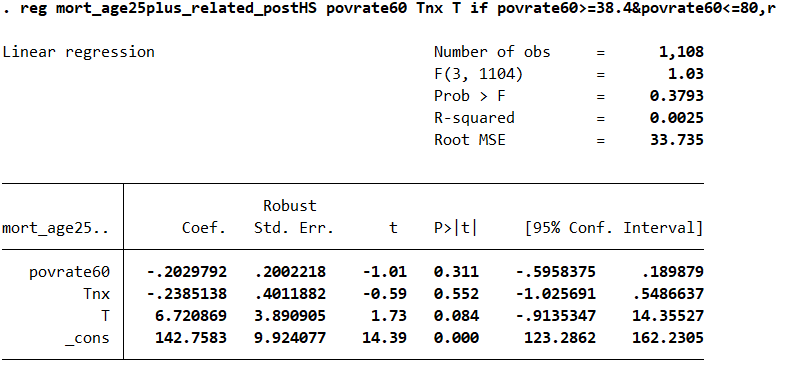
\includegraphics{p12}\\

The above regression outputs show the same robustness tests as in Question 21.8, but for the different x variable. The estimated $\bar{\theta}$ in this case is never significant at the 5\% level, for most of the regressions the estimated p values are quite high. The findings of Ludwig and Miller (2007) pass this check with flying colors.

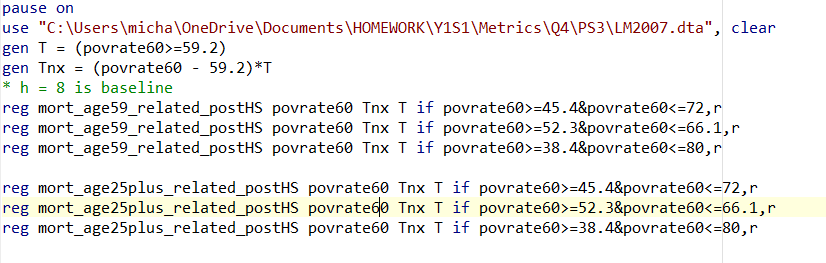
\includegraphics[scale=0.7]{p13}

\end{document}
